\documentclass{article}

\usepackage{amsfonts}
\usepackage[utf8]{inputenc}
\usepackage[english]{babel}
\usepackage{graphicx}
\usepackage{hyperref}
\graphicspath{ {images/} }

\title{Predicting Admissions}
\author{Chinmay Sheth}
 \date\today
%This information doesn't actually show up on your document unless you use the maketitle command below

\begin{document}

\maketitle

\section*{Introduction}

In this exercise, I'm analyzing a university dataset which contains information about student admissions. I am hoping to build a generalized linear model in order to reliably predict a student's admission to the university using SAS.

\section*{Exploratory Data Analysis}

\subsection*{Dataset}

The \href{https://www.kaggle.com/mohansacharya/graduate-admissions}{dataset} that I am using was obtained from Kaggle and it contains data on university admission data. The dataset contains the following columns:

\begin{enumerate}

\item Serial No.
\item GRE Score
\item TOEFL Score
\item University Rating
\item Statement of Purpose Rating
\item Letter of Recommendation Rating
\item Cumulative Grade Point Average
\item Research
\item Chance of Admit

\end{enumerate}

There are nine variables with 400 records, where there are no missing values.

\subsection*{Data Exploration}

There is one categorical variable, Research, which is already encoded as a 0 for no participation in research and 1 for participation in research. The predicted variable of interest is the ninth variable, Chance of Admittance, I am hoping to use a subset of the first eight variables in order to reliably fit a model which is able to explain the variability in the ninth variable well. Furthermore, it doesn't make sense to include the first variable, Serial No., in the basic model because it is random for each student and doesn't effectively convey any meaning.

\section*{Analysis}
\subsection*{Diagnostics}

Through the PROC GLM function, SAS is easily able to build a basic linear model that considers all the variables with interactions, which can be further investigated to determine to see if the linear regression assumption are met. PROC GLM is also able to differentiate between categorical and continuous variables by indicating so in the CLASS definition of the function. As such, "Research" is specified as a categorical variable in the CLASS method. The basic model with interaction terms is as follows: 
\\

$\mathbf{y = B_0 + B_1x_1 +  B_2x_2  +  B_3x_3 +  B_4x_4 +  B_5x_5 +  B_6x_6 +  B_7x_7  +   B_17x_1x_7 + }$ \\ $\mathbf{ B_27x_2x_7 + B_37x_3x_7 +  B_47x_4x_7 +  B_57x_5x_7 +  B_67x_6x_7}$
\\
\begin{enumerate}

\item $\mathbf{y:}$ Chance of Admittance
\item $\mathbf{x_1:}$ GRE Score
\item $\mathbf{x_2:}$ TOEFL Score
\item $\mathbf{x_3:}$ University Rating
\item $\mathbf{x_4:}$ Statement of Purpose Rating
\item $\mathbf{x_5:}$ Letter of Recommendation Rating
\item $\mathbf{x_6:}$ Cumulative Grade Point Average
\item $\mathbf{x_7:}$ 0 if research completed otherwise 1

\end{enumerate}

\begin{figure}
\centering
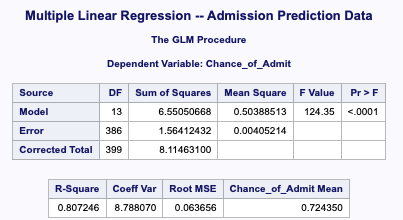
\includegraphics[scale=0.7]{basic_model_output.png}
\caption{Basic model output}
\label{fig:basicmodeloutput}
\end{figure}

After performing the PROC GLM Procedure in SAS, the resulting estimates are displayed in Figure \ref{fig:basicmodelestimate}. The diagnostic plots are checked to see if the regression assumptions are met which are:

\begin{enumerate}

\item $\mathbf{E}(\epsilon_i) = 0$ $ \forall i \in {1..N}$
\item $Var(\epsilon_i) = \theta$ $\forall i \in {1..N}$
\item $\epsilon_i$ are normally distributed $\forall i \in {1..N}$
\item $\epsilon_i$ are independent $\forall i \in {1..N}$

\end{enumerate}


\begin{figure}
\centering
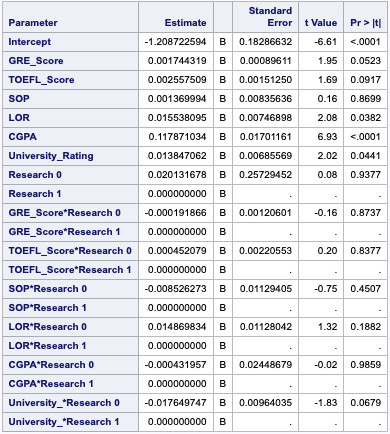
\includegraphics[scale=0.8]{basic_model_estimates.png}
\caption{Basic model estimates}
\label{fig:basicmodelestimate}
\end{figure}

In the diagnostic plots from Figure \ref{fig:basicmodeldiagnostics} there is a departure from the homoskedasticity assumption, that is of constant variance throughout the data, because of the decreasing variance in the data in the Residual vs Predicted Value plot and RStudent vs Predicted Value plot. There also appears to be a departure from the assumption of the expected value of the residuals to equal zero as the data in the two aforementioned plots is not centred around the horizontal zero axis. Finally, the data does not appear to be normally distributed as the Residual vs Quantile Plot shows that the points are not very closely hugging the reference line.

\begin{figure}
\centering
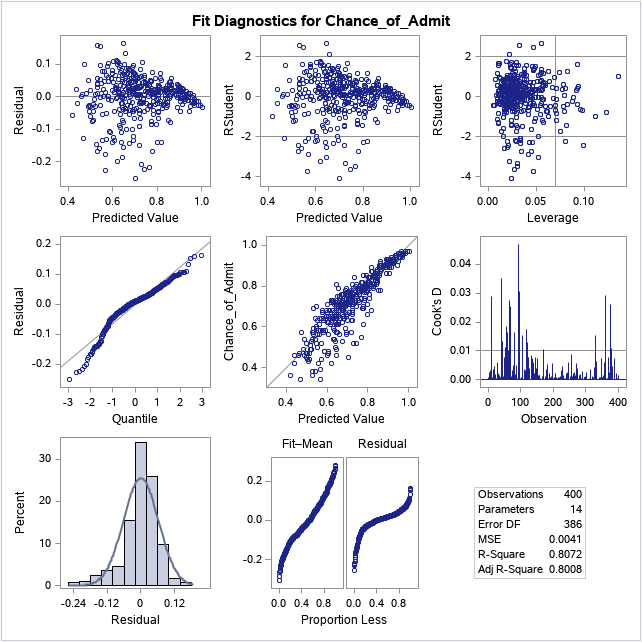
\includegraphics[scale=0.6]{basic_model_diagnostics.png}
\caption{Model Diagnostics for Basic Model with Interactions}
\label{fig:basicmodeldiagnostics}
\end{figure}

\begin{figure}
\centering
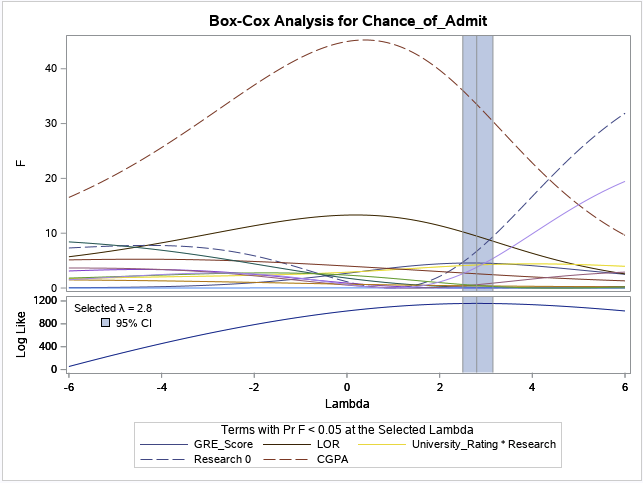
\includegraphics[scale=0.5]{box_cox_analysis.png}
\caption{Box Cox Analysis for Basic Model with Interactions}
\label{fig:boxcoxanalysis}
\end{figure}

\subsection*{Transformations}
Using the data-driven Box-Cox technique, showed in Figure \ref{fig:boxcoxanalysis}, we can estimate the best transformation for the basic linear model which should result in diagnostic plots which have less of a departure from the linear regression assumptions. The R-Squared value has increased from 0.807246 (Figure \ref{fig:basicmodeloutput}) to 0.860190 in the transformed model, indicating that the transformed model is able to explain more variability in the predicted values than the initial model was able to. Furthermore, there appears to be a significantly less departure from the linear regression assumptions as is seen in the diagnostic plots.

\begin{figure}
\centering
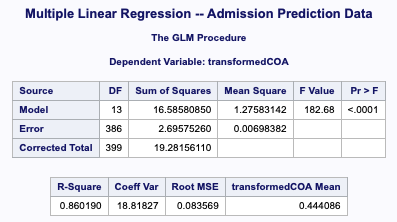
\includegraphics[scale=0.6]{transformed_model_output.png}
\caption{Transformed Model Output}
\label{fig:transformedmodeloutput}
\end{figure}


\begin{figure}
\centering
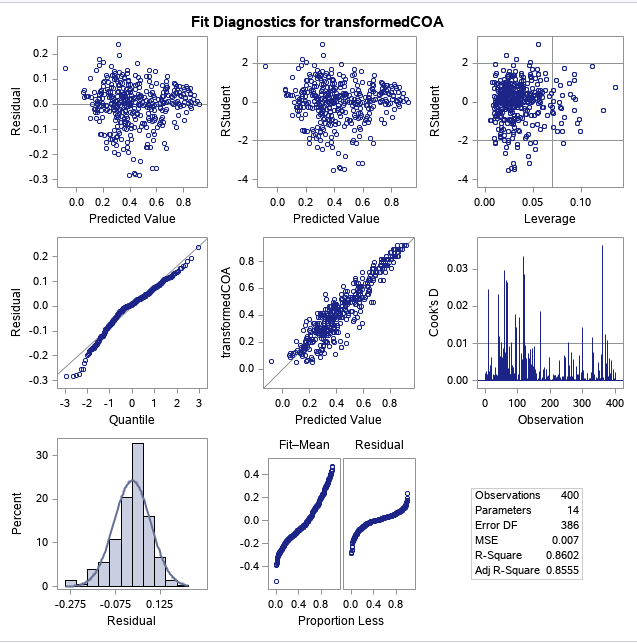
\includegraphics[scale=0.6]{transformed_model_diagnostics.png}
\caption{Transformed Model Diagnostics}
\label{fig:transformedmodeldiagnostics}
\end{figure}

\subsection*{Model Selection}

Now that the regression assumptions have been satisfied, model selection can be performed in order to determine whether all the covariates are truly necessary. According to the \href{https://www.oxfordreference.com/view/10.1093/oi/authority.20110803100346221}{Principle of Parsimony}, we want to be able to explain the variability in the model with the fewest covariates possible, that is, we want to maximize the Adjusted R-squared value while having the fewest number of covariate. In SAS, the GLMSELECT procedure with BIC can be used in order to select the best model. 

The results of this are presented in Figure \ref{fig:bic} which shows that only the following covariates are meaningful to the model:

\begin{figure}
\centering
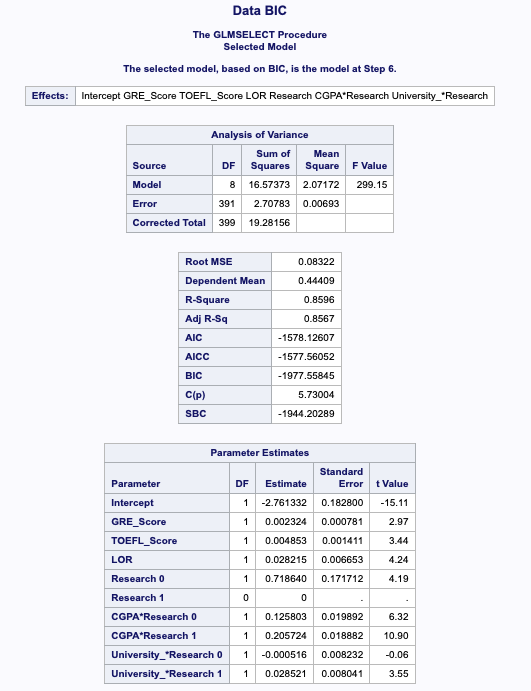
\includegraphics[scale=0.6]{bic.png}
\caption{BIC Model Selection}
\label{fig:bic}
\end{figure}

\begin{enumerate}

\item GRE Score
\item TOEFL Score
\item LOR
\item Research
\item CGPA * Research (Interaction Term)
\item University Rating * Research (Interaction Term)

\end{enumerate}

\section*{Conclusion}

Overall in this exercise, using SAS, we determined that not all of the covariates that were provided were important in model selection. Furthermore, 85.67\% of the variability in the predicted values could be explained with the reduced model that was determined with BIC. The reduced model resulted in an increase in the Adjusted R-Squared value of 4.95\%. 

\end{document}
